% !TeX spellcheck = en_US
% !TeX encoding = UTF-8
\documentclass{beamer}

\mode<presentation> { \usetheme{Madrid} }

\usepackage{graphicx, graphics}
\usepackage{apacite}
\usepackage[style=iso]{datetime2}
\usepackage{enumerate}
\DeclareGraphicsExtensions{.pdf, .png, .jpg, .gif}

\AtBeginSection[]
{
    \begin{frame}
        \vfill
        \centering
        \begin{beamercolorbox}[sep=8pt, center, shadow=true, rounded=true]{title}
            \usebeamerfont{title}
            \insertsectionhead
            \par
        \end{beamercolorbox}
        \vfill
    \end{frame}
}

\title[Periodontitis]{Periodontitis}

\author{Seunghoom Kim \and Jaewoong Lee}
\institute[UNIST]
{
    Ulsan National Institute of Science and Technology
    \medskip
    \newline
    \textit{jwlee230@unist.ac.kr}
}
\date{\today}

\begin{document}
    \begin{frame}
        \titlepage
    \end{frame}

    \begin{frame}
        \frametitle{Overview}
        \tableofcontents
    \end{frame}

    \section{Introduction}
    \begin{frame}
        \frametitle{Microbiome}

        \begin{itemize}
            \item Microbiota: the micro-organisms which live inside \& on humans \cite{microbiome1}
            \item Microbiome: about $10^{13}$ micro-organisms whose which collective genome \cite{microbiome2}
        \end{itemize}

        \begin{figure}
            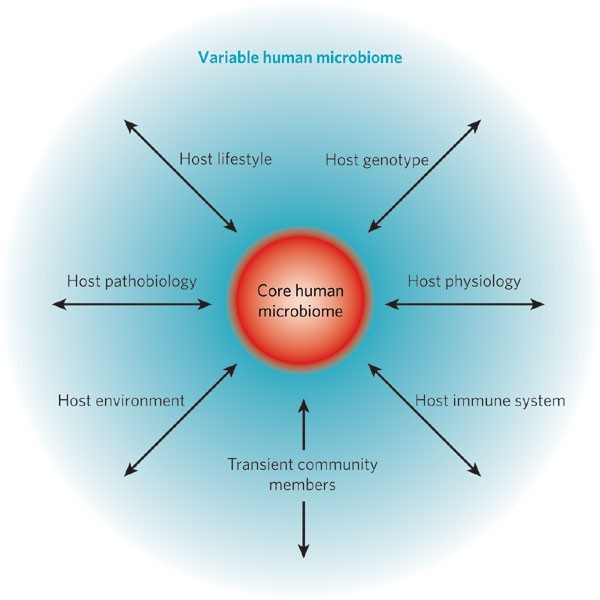
\includegraphics[width=0.3 \linewidth]{figures/microbiome}
            \caption{Concept of a core human microbiome \protected \cite{microbiome1}}
            \label{fig:microbiome}
        \end{figure}
    \end{frame}

    \begin{frame}
        \frametitle{rRNA}

        \begin{itemize}
            \item Ribosomal RNA
            \item Well-known as a key to phylogeny \cite{rRNA1}
        \end{itemize}
    \end{frame}

    \begin{frame}
        \frametitle{Periodontitis (Periodontal disease)}
    \end{frame}

    \section{Materials}
    \begin{frame}
        \frametitle{16S rRNA Sequencing}

        \begin{itemize}
            \item 100 Healthy people
            \item 50 Chronic periodontitis -- Early
            \item 50 Chronic periodontitis -- Moderate
            \item 50 Chronic periodontitis -- Severe
        \end{itemize}
    \end{frame}

    \section{Methods}

    \section{Results}

    \section{Discussion}

    \begin{frame}[allowframebreaks]
        \frametitle{References}
        \bibliographystyle{apacite}
        \bibliography{reference}
    \end{frame}
\end{document}